\documentclass[times,10pt,twocolumn]{article} 
\usepackage{simpleConference}
\usepackage{times}

% Pour la commande onecolabstract (résumé 1 pleine largeur)
\usepackage{abstract}


%\usepackage[margin=2cm, columnsep=20pt]{geometry}
%\usepackage[affil-it]{authblk}
%\renewcommand{\abstractnamefont}{\normalfont\bfseries}
%\renewcommand{\abstracttextfont}{\normalfont\itshape}

% Pour les titres de section/sous-section
%\usepackage[compact]{titlesec}
%\titleformat{\section}{\large\bfseries}{\thesection}{1em}{}
%\titleformat{\subsection}{\normalsize\bfseries}{\thesubsection}{1em}{}
%\titleformat{\subsubsection}{\normalsize}{\thesubsubsection}{1em}{}


%\makeatletter
%\def\@maketitle{%
  %\newpage
  %\null
  %\vskip 2em%
  %\begin{center}%
  %\let \footnote \thanks
    %{\Large\bfseries \@title \par}%
    %\vskip 1.5em%
    %{\normalsize
      %\lineskip .5em%
      %\begin{tabular}[t]{c}%
        %\@author
      %\end{tabular}\par}%
    %\vskip 1em%
    %{\normalsize \@date}%
  %\end{center}%
  %\par
  %\vskip 1.5em}
%\makeatother

\usepackage[french]{babel}
\usepackage[T1]{fontenc}
\usepackage{lmodern}
\usepackage[utf8]{inputenc}
\usepackage{csquotes}

\usepackage[backend=biber, style=nature]{biblatex}
\addbibresource{bibfile.bib}

\usepackage{amsmath}
\usepackage{amssymb}
\usepackage{mathtools}
\usepackage{amstext}
\usepackage{amsthm}
\usepackage{fancyhdr}
\usepackage{siunitx}
\usepackage{physics}

\usepackage{hyperref}


\usepackage{graphicx}
\usepackage{float}
\graphicspath{{figures/}} %Setting the graphicspath
\usepackage{float}
\usepackage{caption}
\usepackage{subcaption}
\usepackage{tabularx}
\usepackage{dcolumn}
\usepackage{booktabs}
\usepackage{makecell}


\renewcommand\thesubsection{\alph{subsection})}
\renewcommand\thesubsubsection{\Roman{subsubsection}}


\newcommand{\angstrom}{\textup{\AA}}
% Astronomy
\DeclareSIUnit\parsec{pc}
\DeclareSIUnit\lightyear{ly}

%Titre
\title{\vspace{-10mm}
\line(1,0){400}\\
Mesure de $H_0$ avec le quasar lentillé \textsc{RXJ1131-1231}
\line(1,0){400}
\vspace{-4mm}
}


%Auteur
\author{\large \textsc{Alexandre Adam}}
%\affil{Département de physique \\ Université de Montréal}
\affiliation{\vspace{2mm} PHY6669 -- Cosmologie\\
Département de physique \\ Université de Montréal
}
\date{\today}

\begin{document}
\twocolumn[
\maketitle
\begin{onecolabstract} % 10 points
\vspace{4mm} %
\end{onecolabstract}
]

\section{Introduction}\label{sec:intro}
\begin{equation}\label{eq:TimeDelay} 
        c\Delta t_{ij} = D_{\Delta t} \left( \frac{(\boldsymbol{\theta_i} - \boldsymbol{\beta})^2}{2} - 
                \frac{(\boldsymbol{\theta_j} - \boldsymbol{\beta})^{2}}{2}
        - \psi(\boldsymbol{\theta_i}) + \phi(\boldsymbol{\theta_j})\right)
\end{equation} 

\begin{equation}\label{eq:Ddt} 
        D_{\Delta t} \equiv (1 + z_{\ell}) \frac{D_\ell D_s}{D_{\ell s}} \propto H_0^{-1}
\end{equation} 
\section{Théorie}\label{sec:theorie}

\begin{equation}\label{eq:Poisson} 
        \grad^{2}_{\theta} \psi = 2 \kappa(\boldsymbol{\theta} )
\end{equation} 

\begin{equation}\label{eq:Potentiel} 
        \psi(\boldsymbol{ \theta}) = \frac{1}{\pi} \int_{\mathbb{R}^2} 
        \kappa(\boldsymbol{ \theta}') \ln(\boldsymbol{\theta} - \boldsymbol{\theta}') d^2\boldsymbol{\theta}'
\end{equation} 

\begin{equation}\label{eq:Convergence} 
        \kappa(\boldsymbol{\theta}) \equiv \frac{\Sigma(\boldsymbol{\theta})}{\Sigma_{\mathrm{cr}}}
\end{equation} 

\begin{equation}\label{eq:Sigcritique} 
        \Sigma_{\mathrm{cr}} \equiv \frac{c^2}{4\pi G} \frac{D_s}{D_\ell D_{\ell s}}
\end{equation} 

\begin{equation}\label{eq:LensEquation} 
        \boldsymbol{\beta} = \boldsymbol{\theta} - \boldsymbol{\alpha}(\boldsymbol{\theta})
\end{equation} 

\begin{equation}\label{eq:DeflectinAngle} 
        \boldsymbol{\alpha}(\boldsymbol{\theta}) = \frac{1}{\pi} \int_{\mathbb{R}^{2}} \kappa(\boldsymbol{\theta}')
        \frac{\boldsymbol{\theta} - \boldsymbol{\theta}^{'}}{|\boldsymbol{\theta} - \boldsymbol{\theta}'|}
        d^{2}\boldsymbol{\theta}'
\end{equation} 

\begin{equation}\label{eq:Kappa} 
        \kappa(\boldsymbol{\theta}) = \frac{3 - n}{2} 
        \left( 
        \frac{\theta_E}{\sqrt{\dfrac{\theta_1^2}{1 - e} + \theta_2^2(1 - e)}}
\right)^{n- 1} 
\end{equation} 
\section{Méthodologie}\label{sec:metho}
\begin{figure}[H]
        \centering
        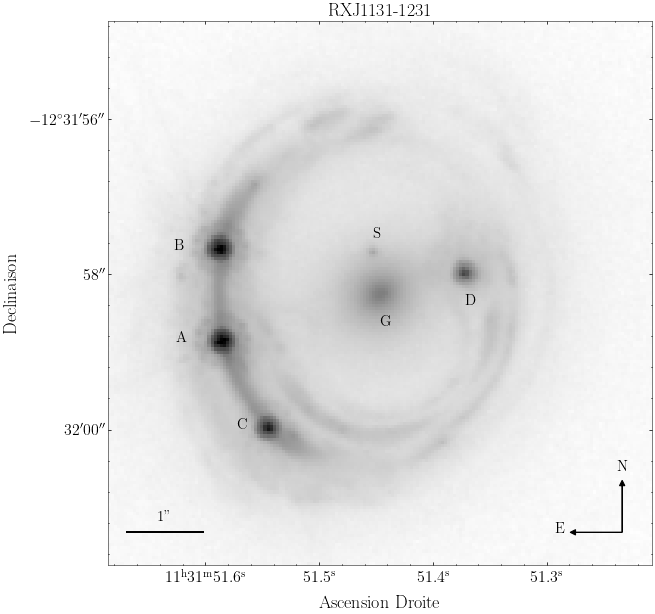
\includegraphics[width=0.8\linewidth]{good_cutout}
        \caption{}
        \label{fig:rxj1131}
\end{figure}

\begin{figure}[H]
        \centering
        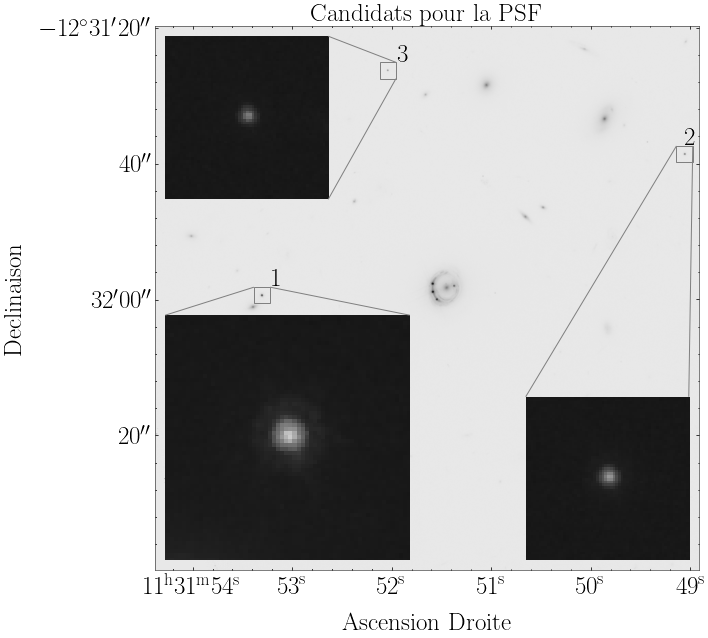
\includegraphics[width=0.8\linewidth]{psf_cutout}
        \caption{}
        \label{fig:psf}
\end{figure}



\begin{align}
        \nonumber
        \log P(\underbrace{\mathbf{d}_{\mathrm{ACS}}}_{\mathcal{D}}
        | \underbrace{\theta_E, e, n, \boldsymbol{\gamma}, \mathbf{\eta}, \mathbf{s}}_{\mathcal{M}}) \propto  
        &-\frac{1}{2}\sum_{i=1}^{|\mathcal{D}|} \frac{(d_{ACS,i} - d_{\mathcal{M}, i})^{2}}{\sigma_i^2}
        \\
\label{eq:Inference} 
        &-\frac{1}{2}\sum_{i < j}^{4} \frac{(\boldsymbol{\beta}_{i} - \boldsymbol{\beta}_i)^{2}}{(d\theta)^{2}}
\end{align} 

\begin{align}
\nonumber
        \log P(\Delta t | D_{\Delta t}, \mathcal{M}) \propto 
        &-\frac{1}{2} \sum_i \frac{(\Delta t_i - \Delta t(D_{\Delta t, \mathcal{M}}))^{2}}{\sigma_{\Delta t}^{2}}
        \\\label{eq:JointLikelihood}
        &+\log P(\mathbf{d}_{ACS} | \mathcal{M})
\end{align}

\section{Résultats et discussion}\label{sec:resultats}
\begin{figure*}[hb]
        \centering
        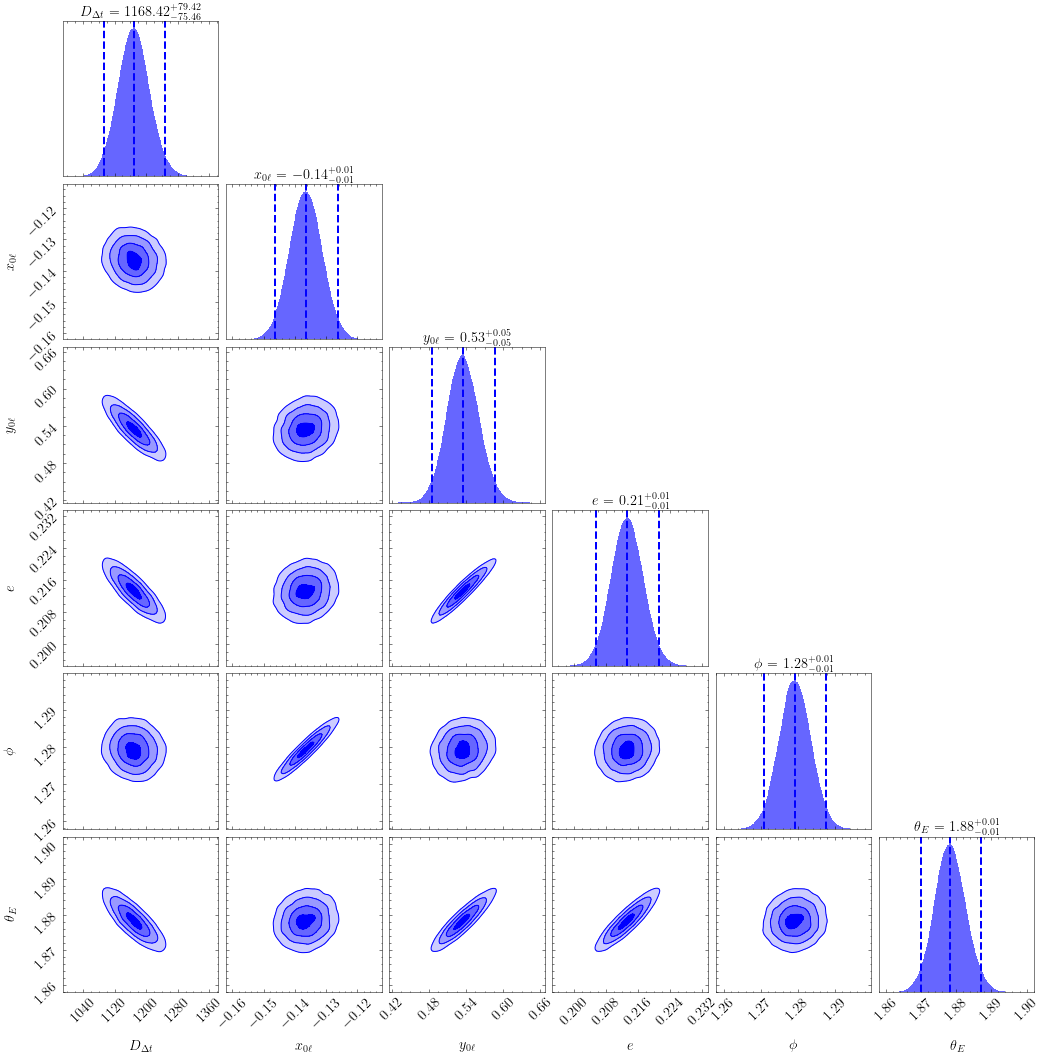
\includegraphics[width=0.8\textwidth]{corner_plot_joint}
        \caption{}
        \label{fig:cornerplot}
\end{figure*}

\begin{figure}[H]
        \centering
        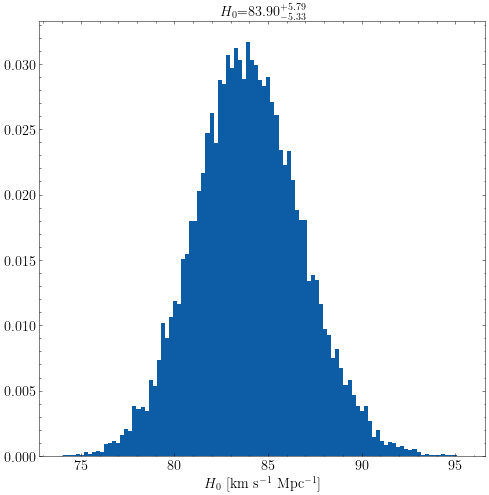
\includegraphics[width=0.8\linewidth]{marginalized_posterior_H0}
        \caption{}
        \label{fig:}
\end{figure}

\begin{table}[H]
        \centering
        \caption{Positions relatives des 4 images du quasar}
        \begin{tabular}{ccc}
                \toprule
                \thead{Images} & \thead{$\theta_1$\\ ($''$)} & \thead{$\theta_2$ \\ ($''$)} \\
                \midrule
                A & 1.8998 & 0.5659 \\\midrule
                B & 1.8717 & -0.6207 \\\midrule
                C & 1.2654 & -1.7385 \\\midrule
                D & -1.3217 & 0.2568 \\
                \bottomrule
        \end{tabular}
        \label{tab:}
\end{table}


\section{Conclusion}\label{sec:conclusion}

\printbibliography

\end{document}

